%
Es soll nun Komplexität des in Abschnitt~\ref{sec:model_developement} entwickelten Modells betrachtet werden. Diese Betrachtung ist wichtig für die Parametrisierung des Optimierungsverfahrens, sowie für eine Beurteilung der generellen Lösbarkeit mit den verwendeten Verfahren. Es wird eine Visualisierung der Fitness-Landschaft\footnote{Auch Fitness-Raum genannt} vorgestellt.\\
%

Um einen Ausschnitt der Fitnesslandschaft zu erstellen, die sog. Fitness-Ebenen, wurde ein eigener Programmteil (der \textit{FitnessPlaneCalculator}) entwickelt. Das Programm nimmt ein in dieser Arbeit entwickeltes Modell, füttert es mit vorgegebenen Daten und schreibt den Rückgabewert in eine Datei. Das Programm lässt sich per Eingabedatei steuern und erlaubt die Definition der Ebenen die dargestellt werden sollen. Es lassen sich immer zwei Variablen der Objektfunktion variieren und der Rest wird dabei auf feste Werte gesetzt. Das erlaubt eine Visualisierung durch eine 2D-Heatmap (siehe folgende Plots). Formal lässt sich das vorgehen wie folgt beschreiben:
%
\begin{equation}
f(\mathbf{x}) \in \mathbb{R}^{N} \rightarrow \mathbb{R}^{2}\nonumber
\end{equation}
%
Aus der Visualisierung können Rückschlüsse auf die Gestalt der Fitnessebene gezogen werden.\\
%

Die Parameter wurden für diese Plots so gewählt, dass sie über einen Bereich iterieren, indem die richtige Lösung liegen sollte. Eingezeichnet sind verschiedene Höhenlinien, die zur Orientierung dienen sollen. Diese sind für die Werte des diskreten Intervalls: $[0,1,5,10,50,100,200]$ ausgeführt. Sie tragen zur besseren Übersicht bei. Die Farbskala das Heatmap skaliert den Plot auf den Wertebereich $[0,1]$ und addiert das im Plot vorkommende Minimum dazu. So kann man leicht eine qualitative Beurteilung der Ebene ablesen. Da nur drei Parameter variiert werden, erhalten die übrigen vier analytisch bestimmte, wahre Werte. Diese sind in Tabelle~\ref{tab:complexity1} zusammen mit den wahren Werten aufgeführt.\\
% In den letzten 2 Sätzen stimmt was nicht: worauf bezieht sich "diese" im letzten Satz?
% Diese = Diese Messwerte?

%
\begin{figure}[h!]
  \caption[Fitness Ebenen Heatmap]{Diese Grafik zeigt die Fitnessebenen $\mathbb{R}^{2}$ des Problems für eine Anordnung aus vier Antennen und einem Sweep über die $x-y$ - Ebene. Jeder Plot ist für einen festen Wert $z$ erstellt worden. In der oberen linken Ecke beginnend und nach rechts laufend. Die $x, y$-Werte wurden über ein Intervall von $[-5,5]$ m und mit einem Inkrement von $0.2$ variiert. Daraus ergibt sich eine für die Abschätzung der Gestalt der Fitnessebene ausreichende Datengrundlage. Die $z$-Werte der $15$-Plots stammen aus dem Intervall $[-7,-7]$ mit einem Inkrement von $1$. Bereits in dieser Ansicht ist zu erkennen, dass der Verlauf sehr Flach ist. Eine Schlucht bildet sich etwa in Nord-Süd-Richtung aus. Jeweils verzeichnet ist das lokale Minima ($+$) eins Plots, sowie die Höhenlinien\footnote{Die Höhenlinien sind für diskrete Werte ${0,1,10,40,50,100,200,500,1000}$ erstellt worden}. Die farbliche Kodierung gibt den Fitnesswert an diesem Punkt an. Die Fitnesswerte wurden normiert und um den Wert ihres Minimums verschoben.}
  \begin{center}
    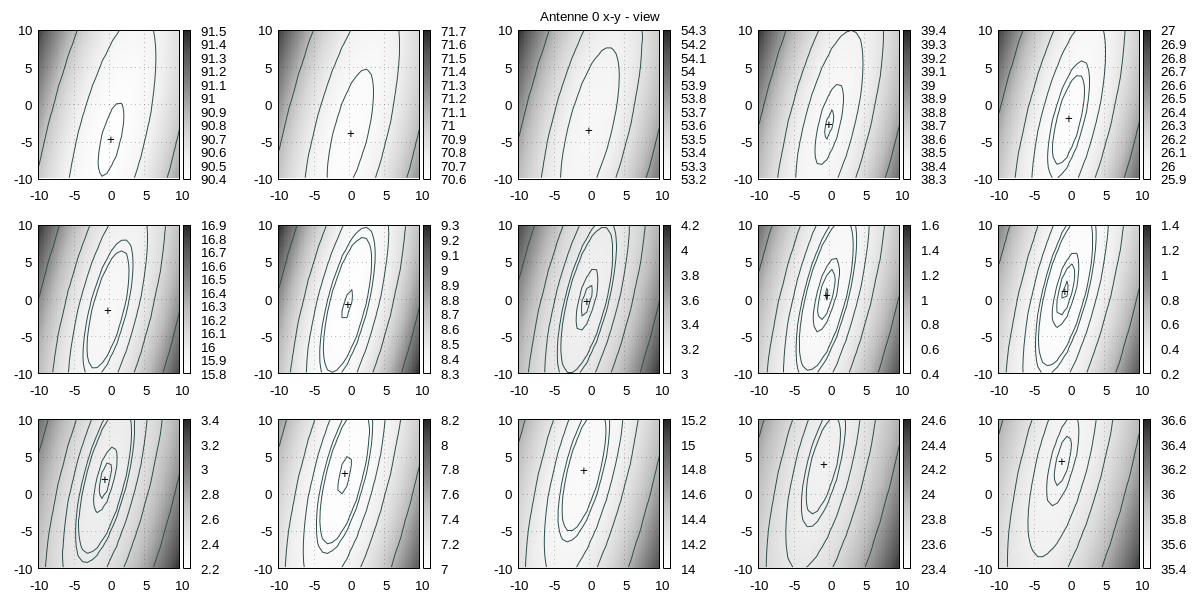
\includegraphics[width=\textwidth]{img/fitness/xy_a0.png}
  \end{center}
  \label{fig:fitnessplane1-x-y-1}
%
\end{figure}

\begin{figure}[ht!]
  \caption[Fitness Ebenen Heatmap, vergrößert]{Vergrößerung der Fitnessebenen der Antenne 1. Es ist hier deutlich zu erkennen, wie gering die Funktionen ansteigen. Das ist ein Problem für die meisten Algorithmen. Es bleibt zu klären wie sensitiv der Algorithmus auf diesen Umstand reagiert. Es wurde um das lokale Minima zentriert und der Bereich auf} % irgendwas normiert? Normierung kann ich in den Grafiken nicht sehen
  \begin{center}
   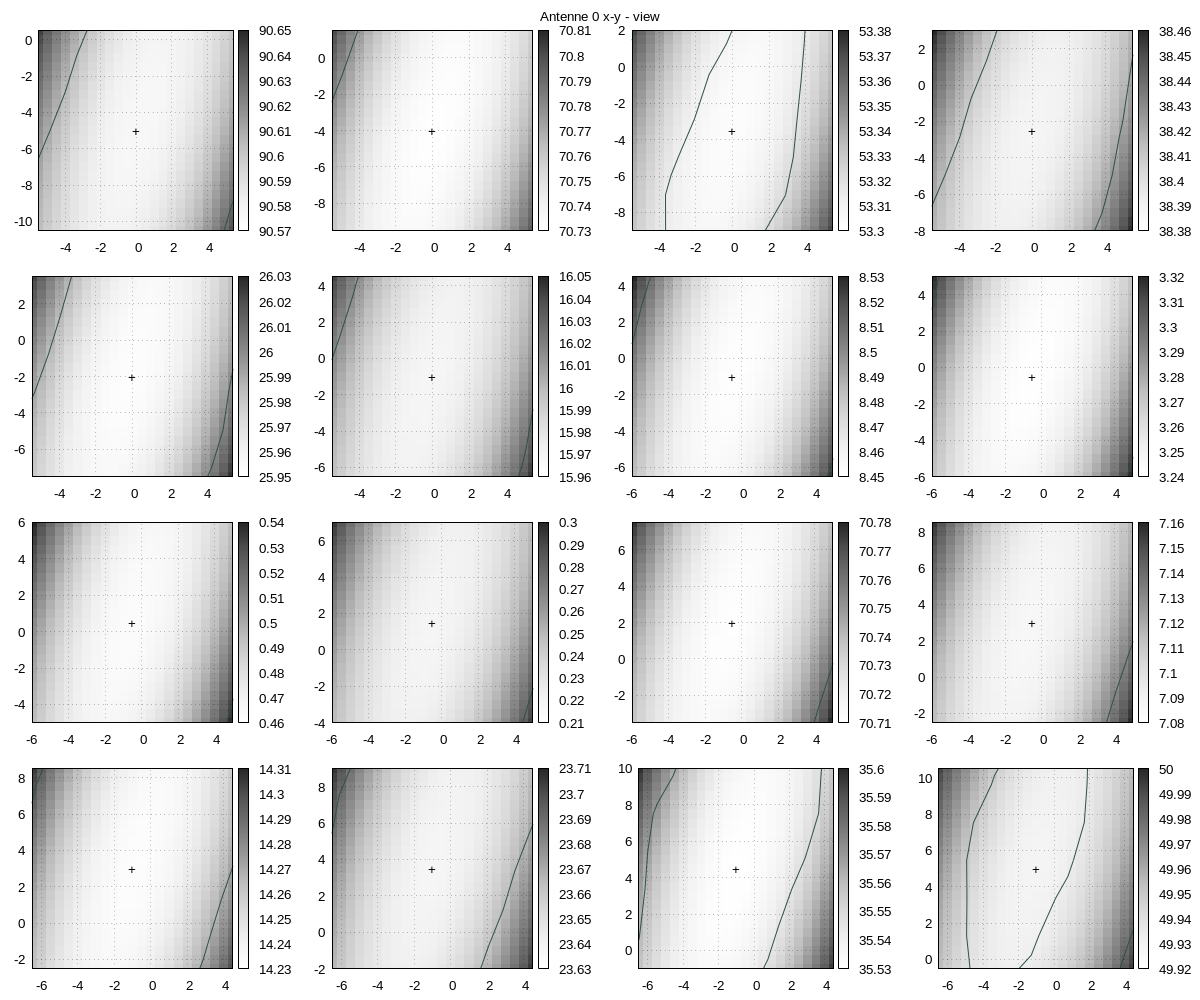
\includegraphics[width=\textwidth]{img/fitness/xy_a0zoomed.png}
  \end{center}
  \label{fig:fitnessplane1-x-y-zoom-1}
%
\end{figure}
%
In den Abbildungen~\ref{fig:fitnessplane1-x-y-1} und \ref{fig:fitnessplane1-x-y-zoom-1} zeigen sich erste Herausforderungen für den Algorithmus. Eine große, sehr flache Fitnessebene für verschiedene Parameter ist nicht leicht zu handhaben. Eine Möglichkeit dieses Problem zu umgehen ist eine große Anzahl an Nachkommen zu generieren. Im Jargon der EA: großes $\lambda$. In den Ergebnissen wurde mit unterschiedlichen Populationsgrößen experimentiert, dabei zeigte sich, dass die Anzahl der Nachkommen groß sein sollte, damit eine gute Güte der Lösung gefunden werden kann. Ein anderer, steuernder Faktor ist die Schrittweite $\sigma$. Diese darf nicht zu klein werden, sonst besteht die Gefahr mit der Population auf der flachen Ebene liegen zu bleibt. Was zu mehrdeutigen Ergebnissen führt. Die Fitness-Ebenen der anderen Antennen zeigen das gleiche Verhalten. Diese sind im Anhang~\ref{app:app:fitness:plots1} zu finden. \\

Aufgrund der Komplexität des in dieser Arbeit erstellten Modells und der Komplexität des zugrunde liegenden Sachverhalts (siehe Abschnitt~\ref{fig:Complexity1}), ist bereits der Fall mit vier Antennen sehr hochdimensional. Er erreicht $7$ Dimensionen und er kann im Rahmen dieser Arbeit nicht vollständig untersucht bzw. dargestellt werden. Die Fitness-Plots aller Antennen und für drei Ebenen sind in Anhang~\ref{app:fitness:plots1} zu finden. Eine vollständige Untersuchung ist indes auch nicht notwendig, da der Algorithmus den Suchraum natürlicherweise untersucht. 
%
\begin{figure}[!h]
	 \caption[Übrige Ebenen für Antenne 1]{Auf diesen Abbildungen zeigen sich die Fitness-Ebenen für die übrigen Ansichten der Antenne 1, x-z und y-z. In der oberen Reihe sind Ebenen über den gesamten Bereich. Die Unteren zeigen eine vergrößerte Darstellung um das Minimum. Zu erkennen ist ein zum Verlauf der x-y-Ebene sehr ähnliches Bild. Ein flaches, längliches Tal mit Minimum. Die Dimension der x-Achse ist [m].} 
	 \label{fig:fitnessplanesA1}
     \centering
     \begin{subfigure}[t]{0.45\textwidth}
             \centering
             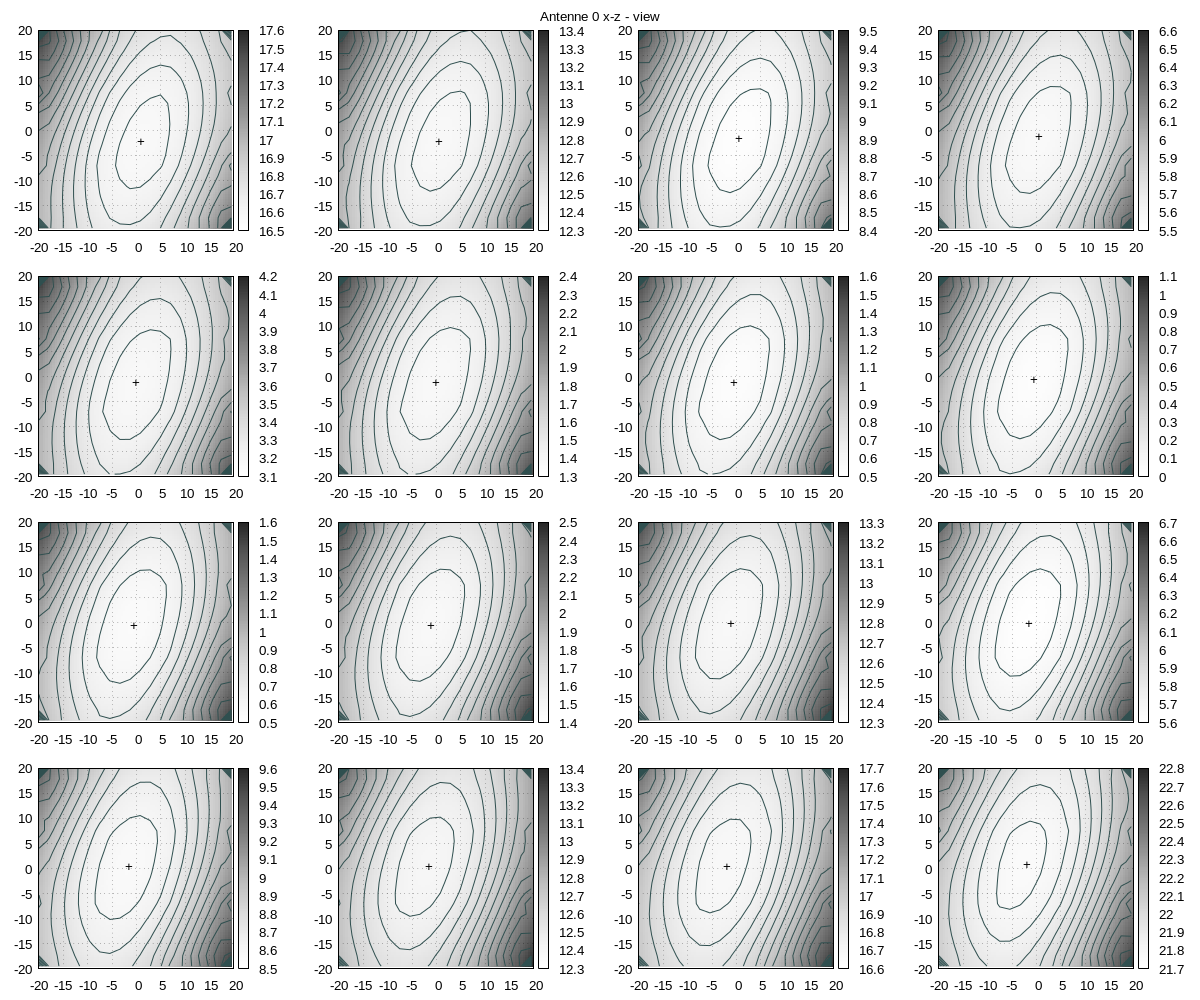
\includegraphics[width=\textwidth]{img/fitness/xz_a0.png}
%             \caption{Statistisch verteilte Endwerte für die Koordinaten der Kalibrierung.}
%             \label{fig:abortedFinal_Calibration_Ant0_ES-boxes}
     \end{subfigure}
     \qquad
     \begin{subfigure}[t]{0.45\textwidth}
			\centering
			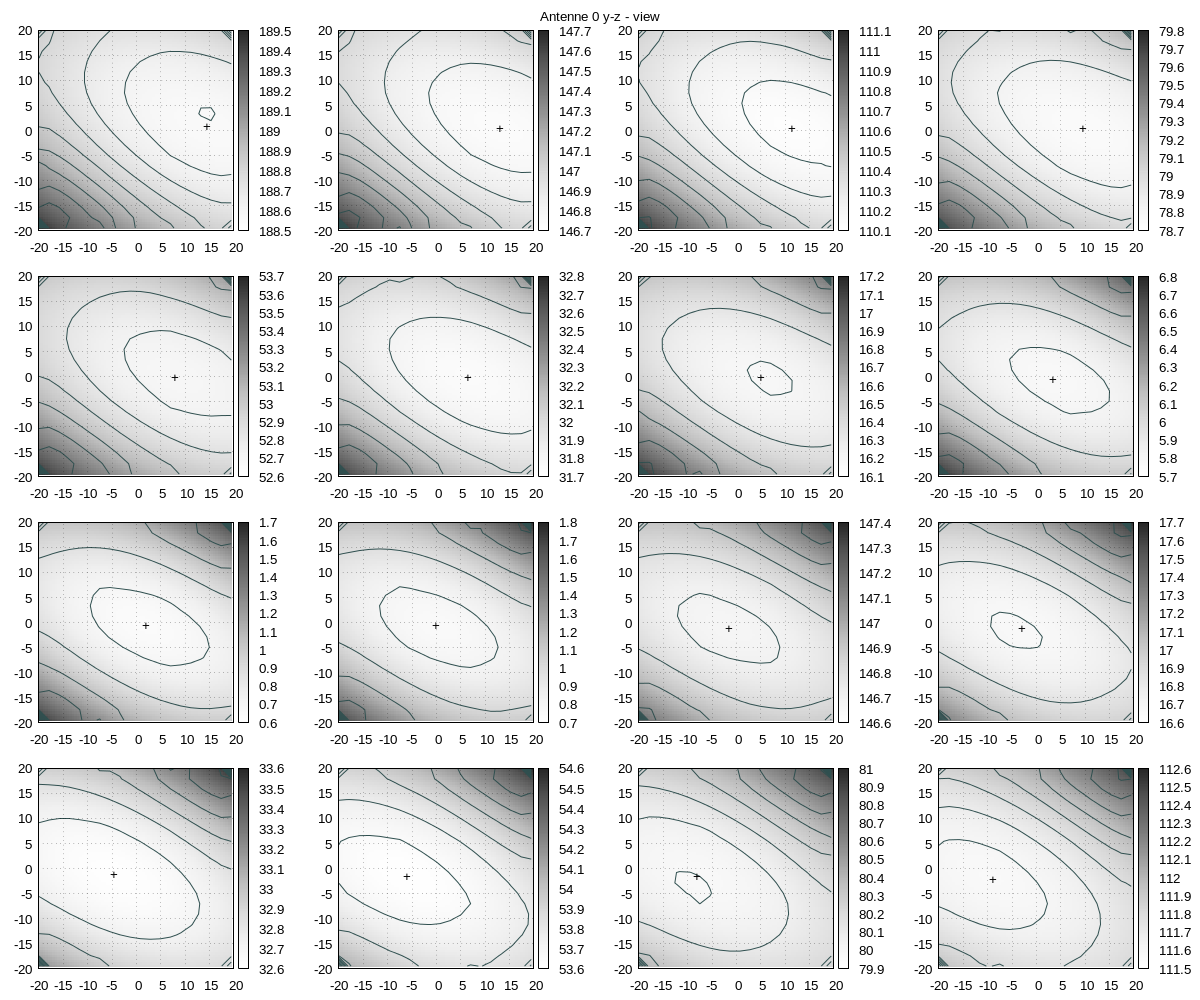
\includegraphics[width=\textwidth]{img/fitness/yz_a0.png}
%			\caption{x-z-Ebene, vergrößert}
%			\label{fig:abortedFinal_Calibration_Ant0_ES-boxes}
	 \end{subfigure}
\\
\vspace{5mm}
     \begin{subfigure}[t]{0.45\textwidth}
			\centering
			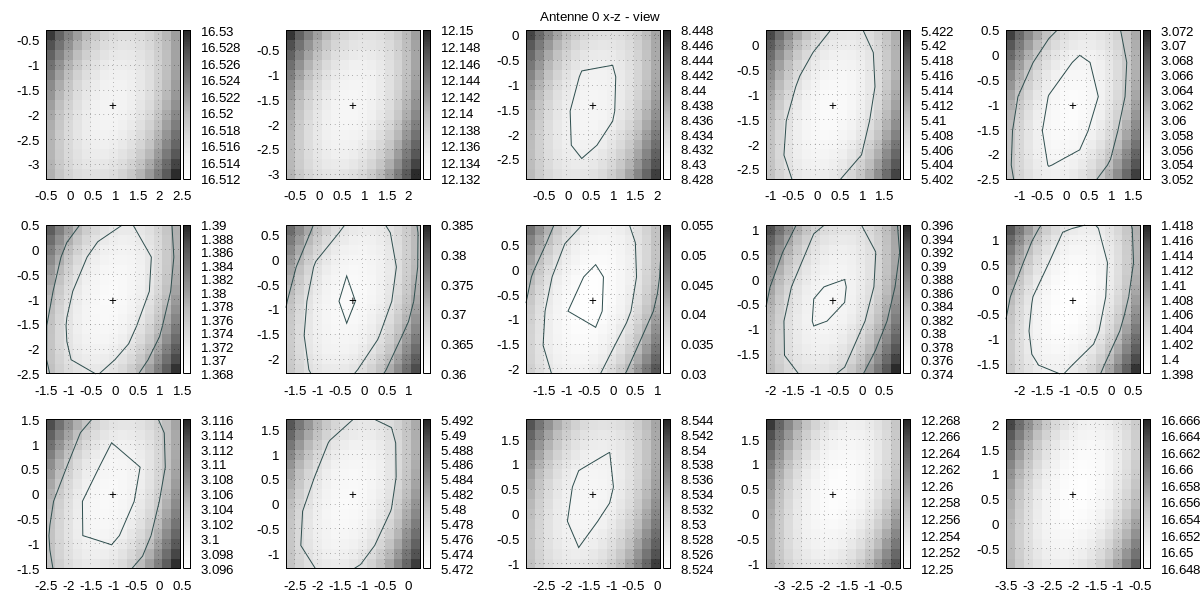
\includegraphics[width=\textwidth]{img/fitness/xz_a0zoomed.png}
%			\caption{x-z-Ebene, vergrößert}
%			\label{fig:abortedFinal_Calibration_Ant0_ES-boxes}
	 \end{subfigure}
	 \qquad
     \begin{subfigure}[t]{0.45\textwidth}
			\centering
			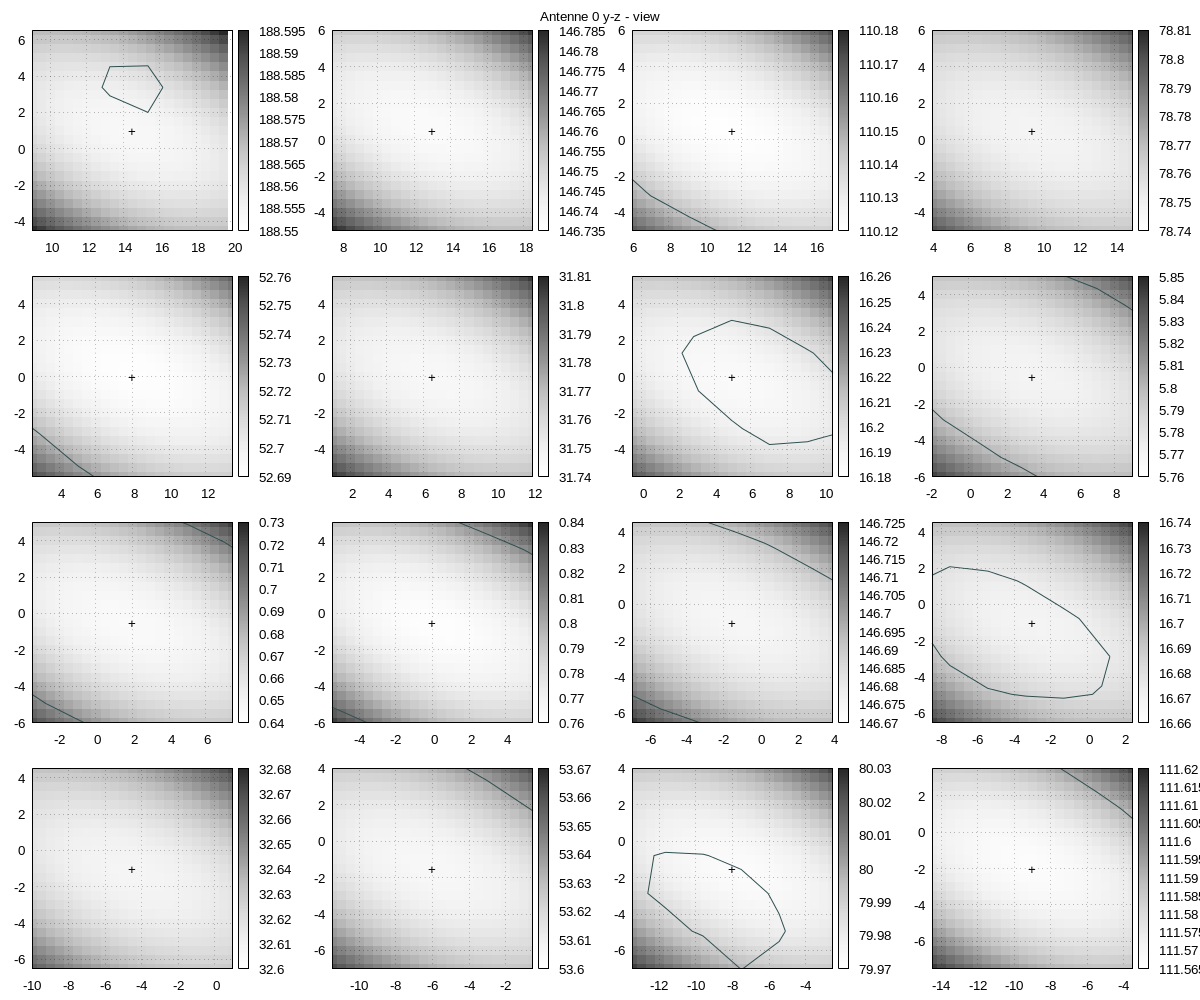
\includegraphics[width=\textwidth]{img/fitness/yz_a0zoomed.png}
%			\caption{x-z-Ebene, vergrößert}
%			\label{fig:abortedFinal_Calibration_Ant0_ES-boxes}
	 \end{subfigure}      
\end{figure}
%
\begin{table} [h]
	\begin{center}
		\caption[Parameter der Fitness Ebenen]{Tabellarisch sind hier die Parameter (Intervalle) der Fitness Ebenen aufgelistet. Zusätzlich sind die Werte angegeben, in denen eine optimale Lösung liegen sollte. Notation: [Start:Inkrement:Ende] }
		\label{tab:complexity1}
		\begin{tabular}{lccccccc}
		\textbf{Ebene} & $\mathbf{x}$ & $\mathbf{y}$ & $\mathbf{z}$ & $\mathbf{n_0}$ & $\mathbf{n_1}$& $\mathbf{n_2}$ & $\mathbf{n_3}$ \\
			\hline
			x-y & [-10:.2:10]		& [-10:.2:10]	& [-7:1:7] & [7:0:7] & [10:0:10]& [13:0:13]&[9:0:9]   \\
			x-z & [-10:.2:10] 	& [-7:1:7] 	& [-10:.2:20] & [7:0:7] & [10:0:10]& [13:0:13]&[9:0:9] \\
			y-z & [-7:1:7]  	& [-10:.2:10]	& [-10:.2:10] & [7:0:7] & [10:0:10]& [13:0:13]&[9:0:9]\\
			\hline
			Wahre & 0.479 & -1.012 & 0.607 & 7  & 10 & 13 & 9			\\
%
		\end{tabular}
	\end{center}
\end{table}